\section{Struct in Rust}



\begin{center}
  \centering
  \begin{minipage}{\linewidth}
    % Primo blocco: 50% dello spazio per il codice
    \begin{minipage}{0.62\linewidth}
      Spesso occorre mantenere unite informazioni tra loro eterogenee. Sebbene sia
      possibile utilizzare una tupla, questa tende a nascondere la semantica del dato:
      una tupla (i32, i32) potrebbe rappresentare una frazione così come le coordinate
      di un pixel, rendendo il codice ambiguo.\newline



    \end{minipage}% <-- IMPORTANTE: il simbolo % qui evita spazi bianchi extra
    \hfill
    \begin{minipage}{0.35\linewidth}
      \begin{minted}[breaklines]{Rust}
struct Player {
  name: String, // nickname
  health: i32, // punti vita
  level: u8, // livello corr.
}
\end{minted}
    \end{minipage}
  \end{minipage}
\end{center}

Quando si intende associare una semantica particolare o legare ad una struttura dati un insieme di
comportamenti, è possibile introdurre una \textbf{struct}.

Una struct è un costrutto che permette di rappresentare un blocco di memoria in
cui sono disposti, consecutivamente, una serie di campi il cui nome e tipo sono
indicati dal programmatore.


Il compilatore capisce quanti byte deve allocare in memoria. Essendo che la memoria è
organizzata a parole (word), per un processore a 64 bit, gli x86, è molto più efficiente
leggere dati che iniziano a indirizzi multipli di 8 byte. Per questo motivo il compilatore
Rust utilizza la tecnica di allineamento e padding.

Se abbiamo una struct composta da un u8 (1 byte) e un u32 (4 byte), il
processore preferirebbe che il u32 iniziasse su un indirizzo divisibile per 4.
Per ottenere questo, il compilatore inserisce dei ``byte morti'' (padding) tra i
due campi.


% prende atto che vi è un nuovo tipo di dato, 
% capendo quanti byte deve allocare
% probabilmente il compilatore decide che al posto di alloare 29byte nel prende 32 dato
% che sono più semplici da gestire a livello di memoria.


% perché i processori non sempre possono leggere byte a byte ad esempio nelgi x86
% può leggere 8bit se l'indirizzo è multiplo di 8.



\subsection{Come utilizzare una struct}

Si istanzia una struct tramite un blocco preceduto dal nome della struttura, contenente
un valore per ciascun campo.

\begin{center}
  \centering
  \mintinline[breaklines]{rust}{let mut s = Player { name: “Mario”.to_string(), health: 25, level: 1 };}
\end{center}


Quando il nome del valore coincide con quello del campo è possibile abbreviare la notazione
stile TypeScript:


\begin{center}
  \centering
  \mintinline[breaklines]{rust}{let p = Player { name, health, level };}
\end{center}

\noindent
\begin{tcolorbox}
  \textbf{Nota:} A differenza del TypeScript, il quale utilizza l'equivalenza strutturale,
  Rust si basa sull'equivalenza nominale. Il tipo Player con 3 valori non ha nulla a che
  vedere con Giocatore con i medesimi campi.
\end{tcolorbox}

\newpage
\subsubsection{Operatore di spreading}

Esiste la notazione di \textit{spreading}, parziale o totale, anche in Rust.\newline

Se è parziale la si può utilizzare solo alla fine:

\begin{center}
  \centering
  \mintinline[breaklines]{rust}{let s1 = Player {name: “Paolo”.to_string(), ..s}}
\end{center}

Se è totale:\newline

\begin{center}
  \centering
  \mintinline[breaklines]{rust}{let s1 = Player {..s}}
\end{center}

\noindent
\begin{tcolorbox}
  \textbf{Nota:} La copia diepnde dai tipi di dati, se posseggono il tratto copy,
  come interi, bool, etc, vengo copiati altrimenti per gli altri dati come le stringhe il
  valore viene mosso e il possesso del dato viene passato alla struct e la
  struct originale s non è più utilizzabile nel suo insieme perché è stata
  parzialmente svuotata.
\end{tcolorbox}


\subsection{Accesso alla struct}

Si accede ai singoli campi con la notazione puntata.

\begin{center}
  \centering
  \mintinline[breaklines]{rust}{println!(“Player {} has health {}”, s.name, s.health );}
\end{center}

Ogni struct introduce un nuovo tipo, il cui nome coincide con il nome della
struct, basato sui tipi che la compongono. Questo permette di disambiguare
l'uso che si intende fare delle singole informazioni contenute.

\subsection{Struct fatte a tupla}

Si possono definire delle struct simili a delle tuple, indicando solo il tipo del campo,
senza attribuire un nome.

Le struct di questo tipo si istanziano come una tupla con l'aggiunta del nome
della struct. Si accede tramite la notazione posizionale.

% Le struct fatte a tupla struct Playground ( String, u32, u32 ); e quetsi cmapi non hanno
% nomi espilici si accede tramite la posizione (notazione posizionale)

\begin{minted}[breaklines]{rust}
struct Playground ( String, u32, u32 );
struct Empty; // non viene allocata memoria per questo tipo di valore

let mut f = Playground( “football”.to_string(), 90, 45 );
//f.1 trovo football
//f.2 trovo 90
//f.3 trovo 45
let e = Empty;  
\end{minted}

La semantica a tupla è adatta in situazioni in cui la semantica del dato è ovvia
e la notazione posizionale risulta più comoda, come ad esempio le coordinate di un punto.
Per il resto, non vi è differenza se non la leggibilità del codice.

% che senso ha? uste in situazioni rare in cuui la semantica del adato è ovvia e la
% notazione posizione è più comoda. vedi le corrdinarte dei punti. per il resto non
% vi è differenza se non la leggibilità per il programmatore.

In Rust è possibile definire anche struct vuote, senza campi. Questi tipi di struct
non occupano spazio in memoria e vengono utilizzati principalmente come marcatori o
per implementare comportamenti specifici tramite il tratto asseganto.


% Rust riesce ad allocare cin tipo che non contiene nulla all'interno. Mi basa il marcatore
% è parente stretto dell'unit type (), mi servono marcatori distinii per diverse situazioni.



\subsection{Probabile rappresentazione in memoria}

\begin{center}
  \centering
  \begin{minipage}{\linewidth}
    \begin{minipage}{0.50\linewidth}
      \begin{minted}[breaklines]{Rust}
fn main() {
  let p1 = Player {
  name: "Mario".to_string(),
    health: 25,
    level: 1u8,
  };
  println!("{:?}", p1);
}
\end{minted}

    \end{minipage}% <-- IMPORTANTE: il simbolo % qui evita spazi bianchi extra
    \hfill
    \begin{minipage}{0.45\linewidth}
      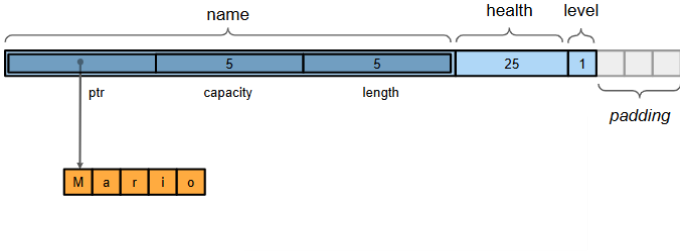
\includegraphics[width=1\linewidth]{images/API_Programming/Tipi-Composti/TC-esempio1.png}
    \end{minipage}
  \end{minipage}
\end{center}


\noindent
\begin{tcolorbox}
  \textbf{Nota:} Non abbiamo garanzia che in memoria sia ordinato nel modo in cui è dichiarato perché
  il compilatore Rust, a differenza del compilatore del C/C++, può riordinare i campi per ottimizzare l'uso della memoria.
\end{tcolorbox}


\subsection{Rappresentazione in memoria}

La disposizione in memoria dei singoli campi è conseguenza di vincoli ed
ottimizzazioni e può essere controllata attraverso opportuni meccanismi.
Ogni singolo campo, in base al proprio tipo, richiede che l'indirizzo a cui
viene collocato sia multiplo di una data potenza di 2 (allineamento).


Rust mette a disposizione la notazione

\begin{center}
  \centering
  \mintinline[breaklines]{rust}{std::mem::align_of_val(...) }
\end{center}
che permette di conoscere l'allineamento richiesto da un particolare valore.
Normalmente è utilizzato internamente per il dialogo con il sistema operativo.

Mentre la funzione

\begin{center}
  \centering
  \mintinline[breaklines]{rust}{std::mem::size_of_val(...) }
\end{center}

ne indica la dimensione in byte occupata in memoria.

Ovviamente i vincoli di allinemanto dipendono dalla piattaforma di esecuzione,
dalla CPU.

\subsubsection{Rappresentazione stile C/C++}

In alcuni casi particolare, come l'interoperabilità con codice C ed altri linguaggi,
interoperabilità con l' hardware, non vogliamo che il compilatore riordini i campi.

A tal proposito viene anteposto alla definizione della struct l'attributo \mintinline{rust}{#[repr(C)]}.


% In std::mem possiamo chiedere dei dettagli. questo tipo che allineamento ha bisogno?
% align\_of\_val ritorna 1 --> qualunque 2 --> pari 4 --> multiplo di 4  8 --> multiplo di 8 etc..
% utilizzato internamento da rust per prendere memoria dal SO

% Anche utile la size\_of\_val() ritorna quanti byte occupa un dato tipo di dato.

\section{Visibilità}

Sia la struct nel suo complesso che i singoli campi che la formano possono
essere preceduti da un modificatore di visibilità.
Per default, i campi sono considerati privati e quindi accessibili nel modulo corrente e nei
sottomoduli, eventuali fratelli o genitori non vedono i campi.

Possono però essere resi pubblici facendo precedere il nome dalla parola chiave pub.\newline


\noindent
\begin{tcolorbox}
  \textbf{Nota:} Posso definire pub solo la sctruct, ma non i campi, in questo caso i campi sono
  privati e non accessibili, come il Vec la cui capacity e size non sono accessibili.
\end{tcolorbox}


Questo permette di implementare il meccanismo di incapsulamento (information
hiding).

% Princpiio dell'incapsulamento (ogniuno a casa sua fa i fatti suoi e gli altri non ci possono mettere becco)

% Ma cosa me ne faccio di uan sgtrcut che ha dei campi che non posso manipolare?
% Posso definire dei metodi per manipolare i campi.

Per essere efficace, occorre però poter associare un insieme di comportamenti
(metodi) alla struct.

A differenza di quanto avviene in altri linguaggi, in cui struttura e comportamento sono definiti
contestualmente in un unico blocco, classe, in Rust la definizione dei metodi associati ad una struct
avviene separatamente, in un blocco di tipo \mintinline{rust}{impl ...}

\section{Metodi}

Rust non è un linguaggio ad oggetti nel senso tradizionale del termine, anche se implementa
incapsulamento e polimorfismo, conseguentemente, non ha il concetto di classe.
Dato che questo concetto tende a creare vincoli non voluti.


% In java vi +è l'erditarietà singola (object) metto dentro has, toString, wait, notifyOne, nnotifYAll, cosa me li faccio,  però intanot ce li hai
% qeusto mi obbliga a definire la classe generatrice.

% In c++ dice non c'è bisogno di creare una classse senza supercalsse, ma puoi creare anche con una superclasse
% ma anche 2 superclassi ereditando da tutti e due. (occhi mamma e braccia pappa)
% Poi c'è il diamond of death.


% Qiuesto ed altro ha portato a portare le persone che scrivono linguaggi
% l'eserditarietà non è il meglio.

% Rust nasce da un bug ad un eseprienza utente non piacevole 28 piani a piedi

% Il creatore dice che è meglio torglersi le classi. ma non i metodi, quindi le struct hanno i metodi


Sebbene le struct possano apparire simili alle classi di altri linguaggi,
il parallelismo è limitato, in particolare, le struct NON sono organizzate in una gerarchia di
ereditarietà. Il concetto di metodo si applica invece a tutti i tipi, compresi quelli primitivi.


Il metodo ha accesso ha a TUTTI i campi della struct, anche quelli privati, questo
ci permette di impelemtnare l'incapuslamento.

\subsection{Definizione di un metodo}
Si definiscono i metodi collegati ad un tipo in un blocco racchiuso tra parentesi
graffe, preceduto dalla parola chiave \mintinline{rust}{impl} seguita dal nome del tipo.


Le funzioni presenti in tale blocco il cui primo parametro sia \mintinline{rust}{self},
\mintinline{rust}{&self} o  \mintinline{rust}{&mut self} diventano metodi.

\textit{Self}\footnote{Corrisponde grosso modo a quello che in altri linguaggi ad oggetti
  viene chiamato this} è una parola chiave che rappresenta l'istanza del tipo di cui si
sta facendo l'implementazione.


Le funzioni che non hanno come primo parametro \textit{self} sono dette funzioni
associate e svolgono il ruolo giocato dai costruttori e dai metodi statici nei
linguaggi ad oggetti.



\begin{center}
  \centering
  \begin{minipage}{\linewidth}
    % Primo blocco: 50% dello spazio per il codice
    \begin{minipage}{0.47\linewidth}
      \begin{minted}[breaklines]{java}
class Something {
int i;
String s;

  void process() {...}
  int increment() {...}
};
\end{minted}

    \end{minipage}% <-- IMPORTANTE: il simbolo % qui evita spazi bianchi extra
    \hfill
    \begin{minipage}{\linewidth}
      \begin{minipage}{0.47\linewidth}
        \begin{minted}[breaklines]{rust}
struct Something {
  i: i32,
  s: String
}
impl Something {
  fn process(&self) {...}
  fn increment(&mut self) {...}
}

\end{minted}
      \end{minipage}
    \end{minipage}
  \end{minipage}
\end{center}

Se in JavaScript il \textit{this} non compare nella lista dei parametri, dato che è implicito,
in Rust viene esplicitato perché dobbiamo dire che operazione facciamo su quel self.

\begin{itemize}
  \item \mintinline{rust}{self}: voglio prendere possesso del ricevitore il quale non sarà più accessibile poi, movimento.
  \item \mintinline{rust}{&self}: chiedo un prestito un sola lettura del ricevutore, posso leggere ma non posso modificali, riferimento condiviso.
  \item \mintinline{rust}{&mut self}: chiedo l'accesso in lettua e scrittura, riferimento esclusivo.
\end{itemize}


% self rappresenta l'istanza. in js usiamo this. qualcosa e nel metodno non cpare nella lista dei parametri
% lo mette il compilatore in automatico. in rust è esplicito, lo devo mettere io perché? perché gli dobbiamo
% dire che operazinoe facciamo sul quel self. eg \&self --> non modifichiamo nulla, \&mut self --> modifichiamo qualcosa, self --> stiamo prendendo possesso dell'istanza (consuma il proprio ricevitore, prendo possesso )
% (self deve essere il primo della serie)
% In entrmbai i casi la prendono a prestitoo


\begin{center}
  \centering
  \begin{minipage}{\linewidth}
    % Primo blocco: 50% dello spazio per il codice
    \begin{minipage}{0.47\linewidth}
      \begin{minted}[breaklines]{rust}
pub struct Point{
  x: i32, //privati
  y: i32,

  impl Point {
    pub fn new(x: i32, y: i32) -> Self {
      Point { x, y }
    }

    pub fn length(&self) -> i32{
      (self.x * self.x + self.y * self.y).isqrt()
    }
}
\end{minted}

    \end{minipage}% <-- IMPORTANTE: il simbolo % qui evita spazi bianchi extra
    \hfill
    \begin{minipage}{\linewidth}
      \begin{minipage}{0.47\linewidth}
        \begin{minted}[breaklines]{rust}
let p1 = Point::new(3, 4);

// possibile solo nello stesso modulo
// o in un sottomodulo di quello in cui
// è stato definito Point
let p2 = Point::new(x:3, y:4);  //potenxilemnte non scrivibile dato che se non sono nello stesso moulo non va bene

let m1 = p1.length(); //5 quando scrivo questo il compilatore traduce in Point::length(&p1)

let m2 = Point::length(&p1); // 5

\end{minted}
      \end{minipage}
    \end{minipage}
  \end{minipage}
\end{center}

I metodi sono funzioni legate ad un'istanza di un dato tipo. Il legame si
manifesta sia a livello sintattico, che a livello semantico.


\paragraph{Sintatticamente} un metodo viene invocato a partire da un'istanza del tipo a cui è
legato utilizzando la notazione \textit{instance.method(...) }

\paragraph{Semanticamente} il codice del metodo ha accesso al contenuto (pubblico e privato)
del ricevitore attraverso la parola chiave self.



\begin{center}
  \centering
  \begin{minipage}{\linewidth}
    % Primo blocco: 50% dello spazio per il codice
    \begin{minipage}{0.47\linewidth}

      \begin{minted}[breaklines]{rust}
struct Point {
  x: i32,
  y: i32,
}
impl Point {
  fn mirror(self) -> Self {
    Self{ x: self.y, y: self.x }  
  }
  fn length(&self) -> i32 {
    (self.x*self.x + self.y*self.y).isqrt()
  }
  fn scale(&mut self, s: i32) {
    self.x *= s;
    self.y *= s;
  }
}


\end{minted}

    \end{minipage}% <-- IMPORTANTE: il simbolo % qui evita spazi bianchi extra
    \hfill
    \begin{minipage}{\linewidth}
      \begin{minipage}{0.47\linewidth}

        \begin{minted}[breaklines]{rust}
fn main() {
  let p1 = Point{ x: 3, y: 4 };
  let mut p2 = p1.mirror();
  let l1 = p2.length(); // l1: 5
  p2.scale(2);
  let l2 = p2.length();
  // l2: 10
}
\end{minted}
      \end{minipage}
    \end{minipage}
  \end{minipage}
\end{center}

\section{Costruttori}

A differenza di quanto capita in altri linguaggi, in Rust non esiste il concetto di
costruttore.

In Rust, invece, qualunque metodo nel blocco \textit{impl}, che ritorna Self, può fare le veci del costuttore.
Questo garantisce che il programmatore sia consapevole delle informazioni contenute al suo interno.


Per convenzione, si sceglie di chiamarlo \textit{new}, ma non è obbligatorio.

\begin{center}
  \centering
  \mintinline{rust}{pub fn new() -> Self {...}}
\end{center}

Poiché Rust non supporta l'overloading delle funzioni, se servono più funzioni di inizializzazione,
ciascuna di esse avrà un nome differente: in questo caso la convenzione è utilizzare un pattern come

\begin{center}
  \centering
  \mintinline{rust}{pub fn with_details(...) -> Self {...}}
\end{center}


\section{Gestione delle risorse}

% All'intero della sturttura datai ci mettiamo le cose che vogliamo gestire, in alcuni casi
% possono avere un significato che va olte la rapp stessa della memoria.

% esempio un numero 42, può esserre un intero ma può essere anche il file handel
% e vorrei fate la close().

Se una struttura contiene al proprio interno risorse la cui semantica richiede una
esplicita gestione del ciclo di vita, occorre fare in modo che, quando la struttura
cessa di esistere, tali risorse siano liberate in modo appropriato. (E.g. file handle, socket, etc.)


Questo compito è affidato ad una funzione speciale detta Drop, il distruttore, il quale se presente viene
chiamato in automatico dal compilatore quando l'oggetto cessa di esistere per liberare le risorse che contiene.

% Drop è il distruttore in Rust. usando impl Drop for type. lo chiama prima di rilasciare la meoria


% Questa cosa che nel costruttore alloco e nel distruttore rilascio è un pattern molto comune, tanto che ha un nome: Resource Acquisition Is Initialization (RAII).


Rust segue il paradigma RAII - Resource Acquisition Is Initialization - l'acquisizione
delle risorse avviene alla creazione, il rilascio alla distruzione.

\section{RAII - Resource Acquisition Is Initialization}

Le risorse sono incapsulate in una classe, struttura, in cui:

\begin{itemize}
  \item il costruttore acquisisce le risorse e stabilisce eventuali invarianti, oppure
        lancia un'eccezione se non può essere fatto
  \item il distruttore rilascia le risorse e NON lancia mai eccezioni
\end{itemize}

Si usano le risorse attraverso l'istanza di una classe RAII-compatibile che ha una gestione
automatica delle durata di tutte le risorse, \textbf{oppure}, ha un ciclo di vita connesso
al ciclo di vita di un altro oggetto (ad es., è parte di esso).


In questo contesto, la presenza della semantica del movimento, garantisce il
corretto trasferimento delle risorse, mantenendo la sicurezza del rilascio.


\section{Distruttori}

Rust gestisce il rilascio di risorse contenute in un'istanza attraverso il tratto Drop,
costituito dalla funzione

\begin{center}
  \centering
  \mintinline{rust}{fn drop(&mut self) -> ()}
\end{center}

Chiamato in automatico dal compilatore.
Si può forzare il rilascio delle risorse contenute in un oggetto usando la funzione
\mintinline{rust}{drop(some_object);} che ne acquisisce il contenuto e determina l'uscita dallo scope.

\begin{center}
  \centering
  \begin{minipage}{\linewidth}
    % Primo blocco: 50% dello spazio per il codice
    \begin{minipage}{0.47\linewidth}

      \begin{minted}[breaklines]{rust}
pub struct Shape {
  pub position: (f64, f64),
  pub size: (f64, f64),
  pub type: String
}

\end{minted}

    \end{minipage}% <-- IMPORTANTE: il simbolo % qui evita spazi bianchi extra
    \hfill
    \begin{minipage}{\linewidth}
      \begin{minipage}{0.47\linewidth}

        \begin{minted}[breaklines]{rust}
impl Drop for Shape {
  fn drop(&mut self) {
    println!("Dropping shape!");
  }
}
\end{minted}
      \end{minipage}
    \end{minipage}
  \end{minipage}
\end{center}


\noindent
\begin{tcolorbox}
  \textbf{Nota:} Il tratto Drop è mutuamente esclusivo con il tratto Copy.
  Se un tipo implementa il primo non può implementare l'altro, e viceversa.
\end{tcolorbox}



\section{Metodi statici}

In C++/Java è lecito inserire all'interno del costrutto \textit{class ....\{ \}} la dichiarazione
di metodi preceduti dalla parola chiave static. Essi non sono legati ad una specifica istanza,
ma possono operare sulle istanze della classe (se neconoscono l'indirizzo)
avendo accesso anche alle componenti private.


In Rust, è possibile implementare metodi analoghi semplicemente non indicando,
come primo parametro, né self né un suo derivato. Questo permette la creazione
di funzioni per la costruzione di un istanza, metodi per la conversione di
istanze di altri tipi nel tipo corrente o, semplicemente, l'accesso a
funzionalità statiche.

L'esempio più comune è il metodo \textit{new}.

\begin{center}
  \centering
  \mintinline{rust}{<Tipo>::metodo(...)}
\end{center}

% Il conscetto di metodo non è presente, se non abbiamo self come parametro o solo costruttoi se ritornano self
% oppure sono metodi statici.

\section{Enum}


In Rust, è possibile introdurre tipi enumerativi composti da un semplice valore
scalare. Ma anche incapsulare, in ciascuna alternativa, una tupla o una struct volta a fornire ulteriori
informazioni relative allo specifico valore.

Anche in questo caso è possibile legare metodi ad un'enumerazione, aggiungendo il blocco \mintinline{rust}{impl ...}
come nel caso delle struct.


\begin{center}
  \centering
  \begin{minipage}{\linewidth}
    % Primo blocco: 50% dello spazio per il codice
    \begin{minipage}{0.47\linewidth}

      \begin{minted}[breaklines]{rust}
enum HttpResponse {
  Ok = 200,
  NotFound = 404,
  InternalError = 500
}
\end{minted}

    \end{minipage}% <-- IMPORTANTE: il simbolo % qui evita spazi bianchi extra
    \hfill
    \begin{minipage}{\linewidth}
      \begin{minipage}{0.47\linewidth}

        \begin{minted}[breaklines]{rust}
enum HttpResponse {
  Ok,
  NotFound(String),
  InternalError {
    desc: String,
    data: Vec<u8> 
  },
}
\end{minted}
      \end{minipage}
    \end{minipage}
  \end{minipage}
\end{center}

Se le struct sono un tipo prodotto perché l'insieme dei valori che può contenere è il prodotto
cartesiano degli insiemi legati ai singoli campi, le enum sono un tipo somma
perché il loro dominio è la somma, l'unione, dei domini dei loro campi. (E.g. o c'è Ok o c'è NotFound o c'è InternalError)

% le enum nella versione elementare sono enumerati con le eotchete 0, 1, 2 al posto di ok, notFound e internal error.

Nelle enum posso legare, oltre che un'etichetta, anche degli altri valori etichetta e non
solo valori numerici associati al valore.
% sono molto interessanre, posso legare oltre che l'etichetta stessa anched ei dettagli ulteriori.

% ok, notFound(string, ), internal error{code: i32, message: String}
% continua ad essere un tipo somma! perchémè una or tra i suoi campi.

\subsection{Rappresentazione in memoria}

In memoria gli enum occupano lo spazio di un intero da 1 byte più lo spazio
necessario a contenere la variante più grande.

% Il compilatore guarda quello chepuò essere il valore più grande + eventualemnte più byte da usare come tag
% ed eventualemnte il padding

% Costtituida da almeno un byte.


\begin{center}
  \centering
  \begin{minipage}{\linewidth}
    % Primo blocco: 50% dello spazio per il codice
    \begin{minipage}{0.6\linewidth}

      \begin{minted}[breaklines]{rust}
enum Shape {
  Square(u32),
  Point(u8, u8),
  Empty,
}
\end{minted}

    \end{minipage}% <-- IMPORTANTE: il simbolo % qui evita spazi bianchi extra
    \hfill
    \begin{minipage}{\linewidth}
      \begin{minipage}{0.35\linewidth}

        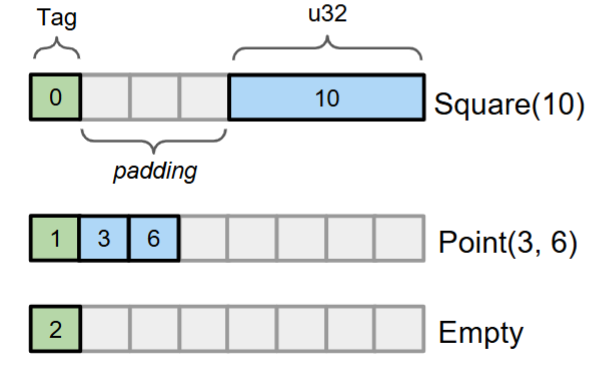
\includegraphics[width=1\linewidth]{images/API_Programming/Tipi-Composti/TC-esempio2.png}

      \end{minipage}
    \end{minipage}
  \end{minipage}
\end{center}


\subsection{Enumerazioni e clausole match}
Il costrutto \textit{match} si presta particolarmente per gestire in modo differenziato
valori enumerativi.

Il comportamento offerto dal pattern matching e la possibilità di legare variabili temporanee in base
alla struttura del valore che viene analizzato offre una sintassi compatta ed efficiente per esprimere
comportamenti alternativi (destructuring assignment).


Il fatto che i pattern confrontati debbano essere esaustivi, garantisce che il codice resti coerente
anche se il numero di possibili alternative presenti nell'enumerazione cambia nel tempo.

\begin{center}
  \centering
  \begin{minipage}{\linewidth}
    % Primo blocco: 50% dello spazio per il codice
    \begin{minipage}{0.35\linewidth}

      \begin{minted}[breaklines]{rust}
enum Shape {
  Square { s: f64 },
  Circle { r: f64 },
  Rectangle { w: f64, h: f64 }
}
\end{minted}

    \end{minipage}% <-- IMPORTANTE: il simbolo % qui evita spazi bianchi extra
    \hfill
    \begin{minipage}{\linewidth}
      \begin{minipage}{0.6\linewidth}

        \begin{minted}[breaklines]{rust}
fn compute_area(shape: Shape) -> f64 {
    match shape {
      Square { s } => s * s,
      Circle { r } => r * r * std::f64::PI,
      Rectangle {w, h} => w * h,
    }
}
\end{minted}
      \end{minipage}
    \end{minipage}
  \end{minipage}
\end{center}


\section{Destrutturazione}

L'utilizzo del pattern matching e la possibilità di destrutturare un valore complesso
non sono limitate al costrutto \textit{match}. È possibile usare la stessa tecnica 
anche all'interno di costrutti di controllo del flusso come:

\begin{center}
  \centering
  \mintinline{rust}{if let <pattern> = <value> ...  }
  e
  \mintinline{rust}{while let <pattern> = <value> ...  }
\end{center}

Tali costrutti verificano se il valore fornito corrisponda o meno al pattern indicato e, nel caso,
eseguono le necessarie assegnazioni alle variabili contenute nel pattern.


\begin{center}
  \centering
  \begin{minipage}{\linewidth}
    % Primo blocco: 50% dello spazio per il codice
    \begin{minipage}{0.47\linewidth}

      \begin{minted}[breaklines]{rust}
enum Shape {
  Square { s: f64 },
  Circle { r: f64 },
  Rectangle { w: f64, h: f64 }
}
\end{minted}

    \end{minipage}% <-- IMPORTANTE: il simbolo % qui evita spazi bianchi extra
    \hfill
    \begin{minipage}{\linewidth}
      \begin{minipage}{0.47\linewidth}

        \begin{minted}[breaklines]{rust}
fn process(shape: Shape) {
  // stampa solo se shape è Square…
  if let Square { s } = shape {
    println!("Square side {}", s);
  }
}
\end{minted}
      \end{minipage}
    \end{minipage}
  \end{minipage}
\end{center}



% Spesso e volentiere vogliamo esaminare cosa è presnte cosa vi è dentro un enum con
% il tag.
% Se sono interessato a capire se ho un quadrato e voglio sapere il lato
% possiamo utilizzare

% if let, voglio gestire solo il quadrato (\_ nel caso avessi matcha
% avrei dovuto utilizzzare anche quell)

La destrutturazione è anche utile per ottenere un “parsing” di una struct, così da
gestirne più facilmente i campi, estraendoli in contenitori singoli da trattare
separatamente. I campi della struct sono "estratti" con il loro nome, direttamente
con l'assegnazione.

% Assegno il valore di shape a Square (s), smonto s con if let "vedi un poi
% se dentro shape cÈè il marcatore square e caccialo nella variabile s.

% Il costrutto if let posso usare anche while let, nella lettura da file,
% posso avere Ok di qualcosa o un error se la lettura è fallita

% while let, la prima voltache ti pianti mollala li e fai altro.

% if let spacchettamento in modo selettivo.

\begin{center}
  \centering
  \begin{minipage}{\linewidth}
    % Primo blocco: 50% dello spazio per il codice
    \begin{minipage}{0.35\linewidth}

      \begin{minted}[breaklines]{rust}
pub struct Point {
  x: i32,
  y: i32
}
\end{minted}

    \end{minipage}% <-- IMPORTANTE: il simbolo % qui evita spazi bianchi extra
    \hfill
    \begin{minipage}{\linewidth}
      \begin{minipage}{0.6\linewidth}

        \begin{minted}[breaklines]{rust}
... 
let p = Point { x: 5, y: 10 };
...
// la destrutturazione deve rispettare i nomi dei campi
let Point { x, y } = p;

println!("The original point was: ({},{})", x, y);
\end{minted}
      \end{minipage}
    \end{minipage}
  \end{minipage}
\end{center}


% Il concetto di destrutturazione può essere anche applicato ad oggetti al di
% fuori di enum.

% Eg una struct, non ho dubbi sui campi interni, non può fallire
% e non uso if let ... ma uso direttameente l'asseganzione.


% Se il dato ha tratto copy manntengo accessibile l'originale, altrimenti
% il valore viene trasferito assieme al possesso dell'owner oriniale.

Il processo di destrutturazione utilizza la semantica delle assegnazioni. Se il valore 
implementa il tratto copy, le variabili introdotte nel pattern conterranno una copia
dell'elemento corrispondente. In caso contrario, verrà eseguito un movimento, 
invalidando il valore originale.

\begin{minted}[breaklines]{rust}

enum Shape{
  Square{s:f64}, 
  Circle{r:f64}, 
  Rect{w:f64, h:f64}
}

impl Shape{
  fn area(&self) -> f64{
    match self{
      Shape::Square{s: &f64} => s * s,
      Shape::Circle{r: &f64} => std::f64::PI * r * r,
      Shape::Rect{w: &f64, h: &f64} => w * h,
    }
  }
}

fn main() {
  let s = Shape::Square { s: 3.0 };
  println!("Area: {}", s.area());
}

fn shrink_if_circle(shape: &mut Shape) {
  if let Shape::Circle { r } = shape { *r *= 0.5}; //r ha tipo &mut f64
}
  
\end{minted}

% posso legare i metodi alla mai enum.


% Noi un tipo di ennum l'abbbiamo già inccontrata, è il Result<T, E>.

% Questo ci porta a parlare di un altro concetto molto importante,
% quelllo della gestione degli errori.



